\section*{Question 3}
(1) A training function was used to implement the algorithm described above in the previous question. The function returns optimal values of $b$ and $\theta$ such that $F_{\lambda}$ is minimized. These parameters were then used to predict the classes for both the training data and the testing data provided. After classification, the error was calculated as the fraction of incorrectly classified samples in the dataset. For $\lambda = 5/\sqrt{N}$, the training and testing errors were calculated to be 0.230 and 0.202, respectively. From observing the optimal value of $b$, there is only one non-zero coefficient at the (3, 1) index. 

(2) The algorithm was also run on larger training and testing datasets for various values of $\lambda$. The total number of iterations required ($i_{total}$), the number of non-zero coefficients in each column of $b$ ($bnz_{1}, bnz_{2}$), and the rates of correct classification on both the training set ($RCC_{train}$) and the testing set ($RCC_{test}$) for each case are all shown below in Table 1. A plot of the cost function after each minimization step for specific values of lambda is shown below in Figure 1. The total number of iterations that is listed contains all the iterations for the BFGS and SLSQP algorithms within the alternating minimization steps.
\begin{table}
\centering
 \begin{tabular}{||c c c c c c||} 
 \hline
 $\sqrt{N}\lambda$ & $i_{total}$ & $bnz_{1}$ & $bnz_{2}$ & $RCC_{train}$ & $RCC_{test}$ \\ [0.5ex] 
 \hline\hline
0.1 & 32 & 29 & 27 & 0.847 & 0.791 \\
0.5 & 165 & 19 & 21 & 0.848 & 0.801 \\
1 & 147 & 12 & 16 & 0.845 & 0.807 \\
2.5 & 188 & 3 & 4 & 0.832 & 0.813 \\
5 & 222 & 3 & 3 & 0.843 & 0.825 \\
7.5 & 284 & 2 & 3 & 0.852 & 0.835 \\
10 & 226 & 2 & 2 & 0.853 & 0.834 \\
20 & 319 & 2 & 1 & 0.848 & 0.834 \\
30 & 238 & 0 & 0 & 0.790 & 0.770 \\ [0.5ex] 
 \hline
 \end{tabular}
 \caption{Results from the minimization algorithm for various values of $\lambda$}
\label{table:1}
\end{table}
\begin{figure}
    \centering
    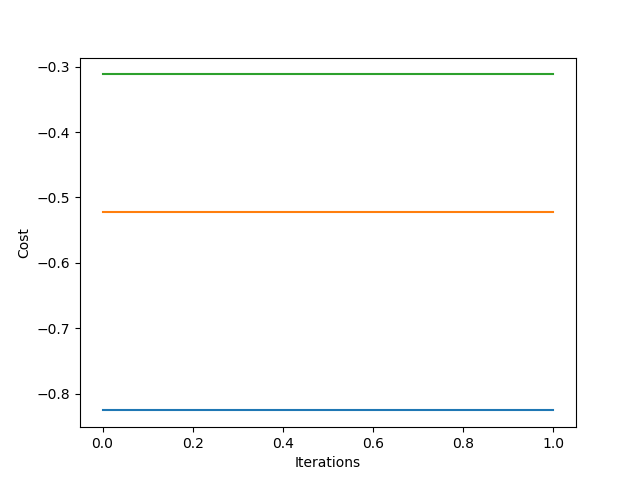
\includegraphics[height=4in]{Figure.png}
    \caption{Cost function after each minimization step for different values of $\lambda$. The blue, orange, and green lines represent $\sqrt{N}\lambda$ = 0.1, 5, and 10, respectively.}
\end{figure}

It is important to note that the program may have errors. The cost function does not appear to have been minimizing and as a result, the overall algorithm for most of the cases only ran once; this is observed in Figure 1. However, the optimal values for b still appear to be unique and can effectively classify most of the test data. The program that was used to generate the parameters is attached with this assignment.